\subsection*{Borealis}
\label{sec:borealis}

\paragraph{Overview}
Borealis~\cite{borealis-design} is a distributed stream processing engine developed at MIT, Brandeis and Brown. 
The core of the system is derived from a previous project called Aurora. This was a centralized version of the stream 
processing engine which was then evolved into a distributed version called Medusa.
Borealis stems from the experience of these two projects extending their functionalities to become a true distributed
stream processing system.

\paragraph{Query Model}
Borealis employs a \emph{boxes-and-arrows} model to express queries, which is derived directly from the one used in
Aurora. Instead of using a relational approach as CQL, it opted for a more graphical representation.
%operators
Operators are boxes, connected by arrows indicating the communication channels among them. The set of operators
supported is also different than the typical SQL one, even though equivalent. Supported operators are divided into two
categories, stateful and stateless. The first group needs more than one tuple to operate, like aggregate, to calculate
an aggregate function over a window of tuples, and Join, similar to the traditional SQL join. Stateless operators operate
on one tuple at the time. This group includes Map, to modify some fields in a tuple, Union, to merge multiple streams
and Filter, which routes tuple according to some condition. The complete set of boxes includes also some other minor
operators and users can develop their own custom ones to suit their needs.

\paragraph{Consistency Model}
Borealis adopts a strict consistency model which aims at eventual consistency. This means that in case of tuple loss or
misordering, the system always tries to obtain the correct final result. It achieve this by marking as \emph{tentative}
a stream on which an error has occurred.  Later it tries to restore the correct result by employing a revision process
which allow the final result to be correct.  This, of course, assumes a scenario where fault is more an exception than
the rule, as the cost for this revision process can become really high. There is no mechanism to quantify the error to
the user. As the error is thought to be transient and recoverable the only feedback given is that the stream content is
invalid and cannot be trusted until recovery. We developed a quality-centric data model that allows the system to
quantify the impact of the error and to provide the user with better feedback on the actual performance of the system.
The revision mechanism used in Borealis also allow to perform ``time travel''.  It means that it's possible to
recalculate tuples of the past and even in the future, by providing a prediction formula. Rolling back to a past
configuration is a heavy-duty process and needs a large amount of storage which is not always feasible due to the nature
of stream processing. Figure~\ref{fig:borealis-fault_tolerance} shows a state machine depicting the fault tolerance
mechanism employed by Borealis. 

\paragraph{Dynamic Query Modification} Borealis also acknowledges the need for dynamic query modification, especially on
long running queries~\cite{borealis-load}. During the execution of query many factor can influence its behavior. For
example the rate of base streams can increase or the load on the allocated machines can become can increase. In this
cases it is important to be able to modify the query on the fly without having to disrupt and recreate it. In Borealis
this is possible by accessing the catalog~\cite{borealis-catalog}, which keep track of which operators are running and
where. In case of node overload, for example, it is possible to place a load-shedding operator to reduce the rate of
incoming tuples, or to migrate the operator all together.

\paragraph{Considerations}
Also, the logging of all data, at sources or at proxies, combined with the necessity of reconciling the
state of all replicas is extremely expensive and poses serious scalability issues. 

\begin{comment}
\begin{figure}[h!]
	\centering
	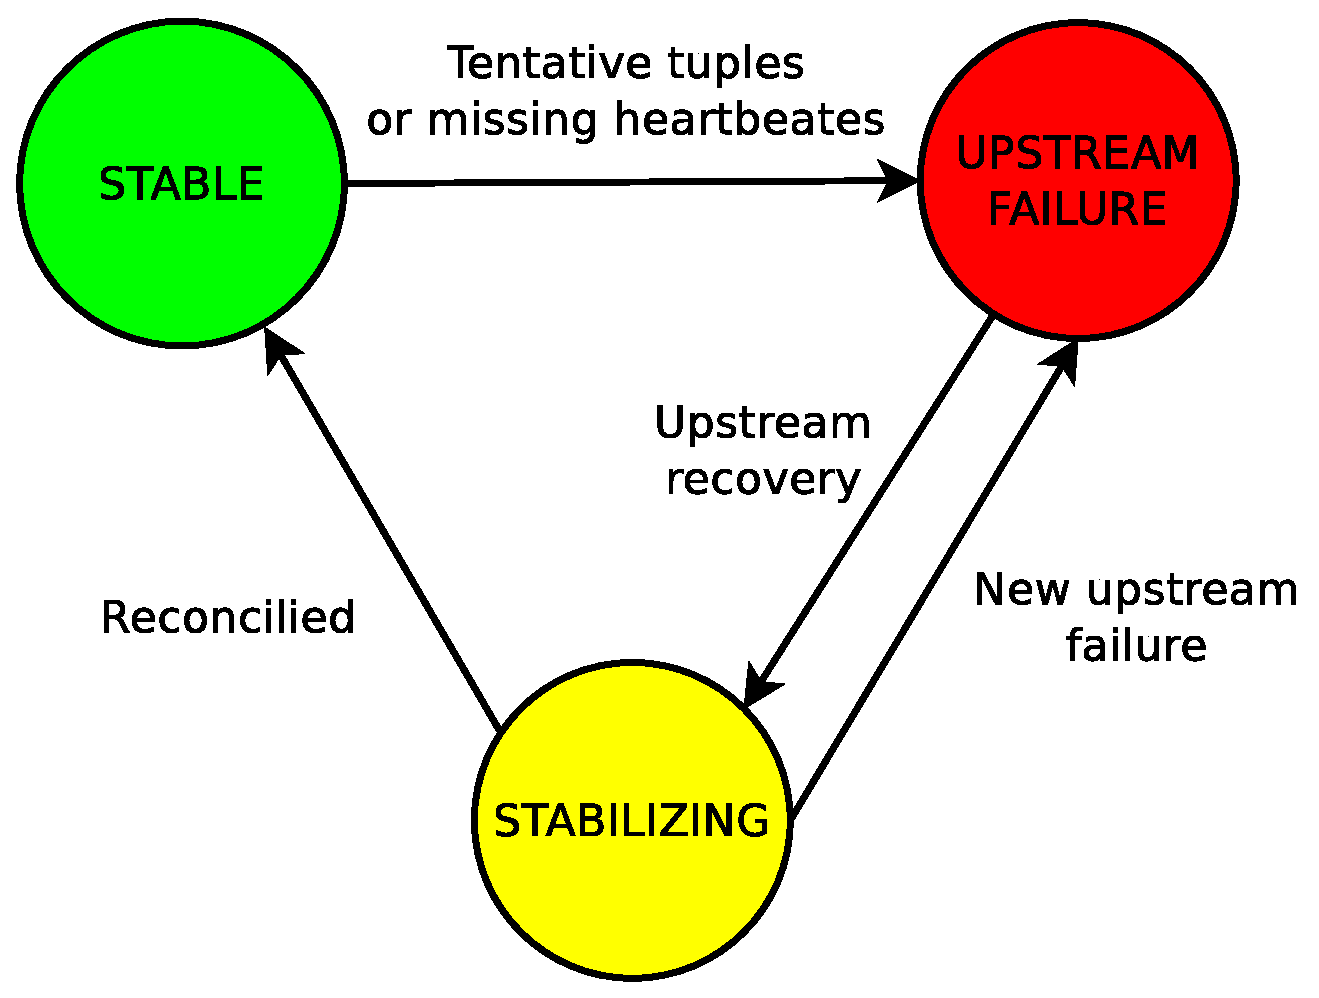
\includegraphics[width=.5\textwidth]{img/borealis-fault_tolerance}
	\label{fig:borealis-fault_tolerance}
	\caption{State machine describing Borealis fault tolerance mechanism. When failure occurs upstream an operator is
alerted by the receival of tentative tuples or by the lack of heartbeat messages. It then marks his tuples as tentative,
while waiting for stabilization. In the end, the failure is overcome, the state is reconciled and the system becomes stable once again.}
\end{figure}

\end{comment}
